% !TeX root = ../../../main.tex
\subsubsection{Results: ATE Estimation}
\label{ch03:sec:04_results_causal}
% \vspace{-0.25em}

Tables~\ref{ch03:tab:table_ate_3_6} and~\ref{ch03:tab:table_ate_9_12} present the Average Treatment Effect (ATE) estimates for non-adherence at 3, 6, 9, and 12 months\footnote{Appendix~\ref{ch03:adp:from_assoc_to_causal} outlines the assumptions required for causal interpretation of our results.}.
Negative ATE values indicate that non-adherence is associated with a shorter adverse event time (i.e., an earlier occurrence of an adverse event) compared to adherence.
Figure~\ref{ch03:fig:graphical_ATE_trend} shows the ATE trends for each method across time snapshots.

Several key observations emerge from the ATE estimates. 
At early time points (3, 6, and 9 months), most models indicate that non-adherence is associated with earlier adverse events, with ATE estimates generally ranging from -0.5 to -4 months. 
Matching-based estimators tend to yield the most negative estimates, reinforcing the association between non-adherence and a shorter time to adverse event. 
The Causal Survival Forest (CSF) provides relatively stable estimates, consistently showing a negative ATE.

DeepHit exhibits high variability in its ATE estimates, sometimes producing values that deviate significantly from those of other models. 
Notably, at 6 months, DeepHit reports an ATE of \(11.551 \pm 3.806\), far from the estimates given by other methods. 
This instability aligns with its poor performance in survival analysis, where it consistently showed the lowest \(C^{td}\) and \(\text{AUC}^{td}\) scores and the highest IBS values.

In contrast, Random Survival Forest (RSF) not only achieves strong predictive performance in survival analysis but also provides more stable ATE estimates, consistently reporting negative values across time points, aligning with broader trends observed in other models. 

The negative ATE estimates at early time points align with clinical expectations that sustained medication adherence can stabilize patients with severe mental illness, thereby reducing the risk of crisis events.
Additionally, robust models such as RSF and CoxPH produce relatively consistent ATE estimates across different causal estimation approaches, including T-learners, S-learners, and matching-based estimators.
This consistency further supports the reliability of these estimates.
However, despite adjustments using demographic variables and county-provided risk scores, residual time-varying confounding may still influence these estimates, suggesting a need for more advanced causal modeling approaches that explicitly account for dynamic adherence and confounding effects.


% !TeX root = ../../../main.tex
\begin{figure}[!ht]
\ChThreeFloatContents
  {ch03:fig:ite_injectable}
  { \caption{
  Distribution of Estimated Individual Treatment Effects (ITE) for different medication adherence groups: \textcolor{ChThreeForestGreen}{injectable}, \textcolor{orange}{non-injectable}, and \textcolor{purple}{not covered} at time snapshot \(\tau=3\) months. 
    Each plot's legend highlights the Average Treatment Effect (ATE) in months for the groups covered by \textcolor{ChThreeForestGreen}{injectable} medication, \textcolor{orange}{non-injectable} medication, and those \textcolor{purple}{not covered} by any medication. 
  (a)-(c): T-learner ITEs for CoxPH, DeepSurv, and Random Survival Forest. 
  (d): ITE for Causal Survival Forest.}}
  {%
    \subfigure[\footnotesize (CoxPH, T-Learner)]{\label{ch03:fig:ite_injectable_coxph}%
      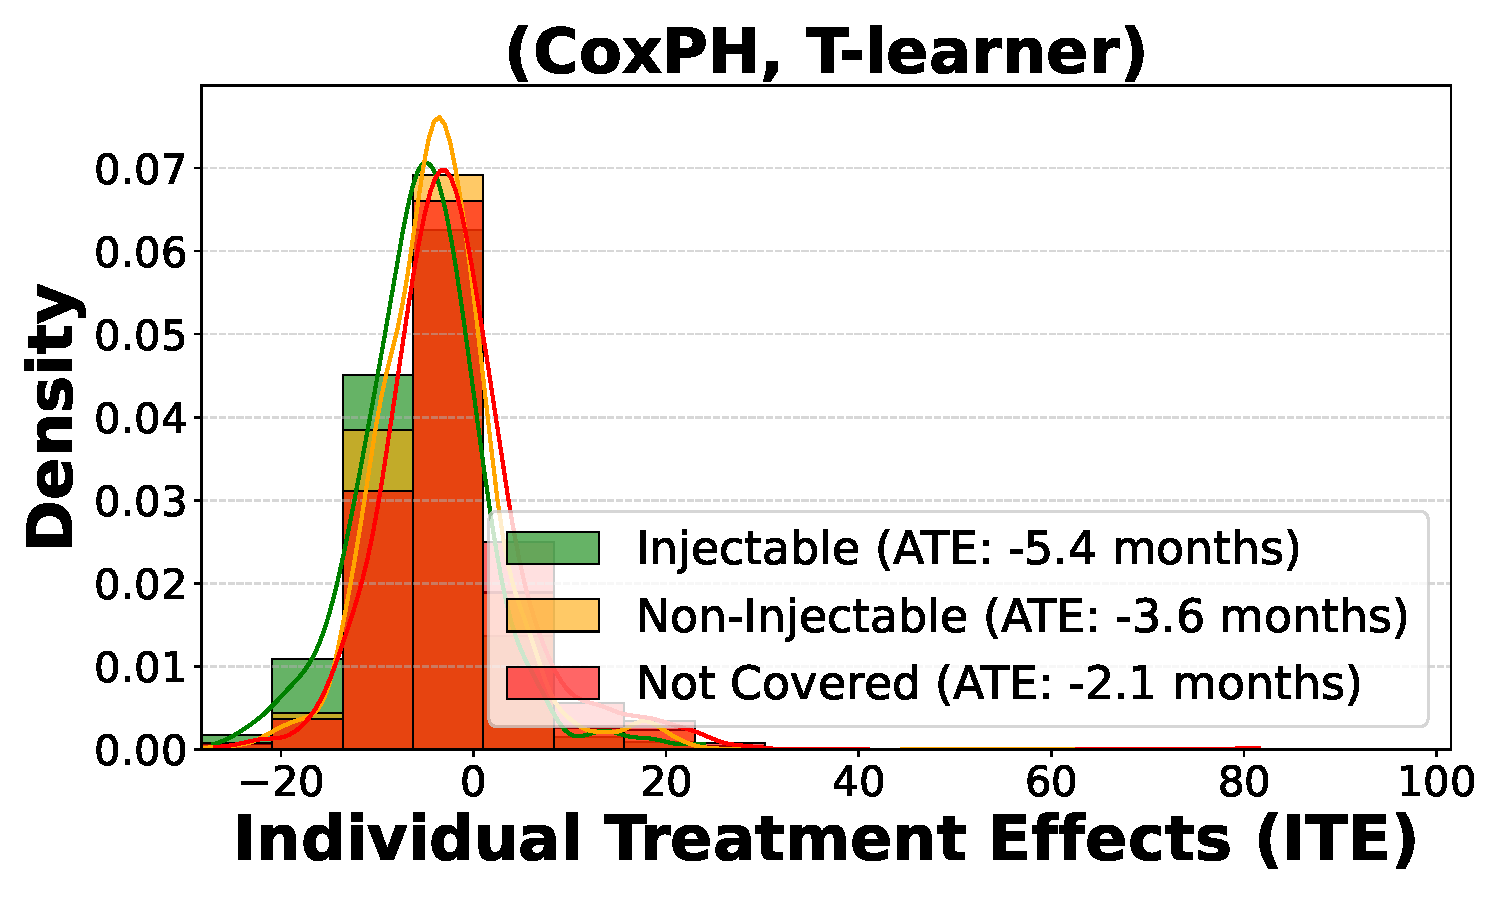
\includegraphics[width=.22\linewidth]{Chapters/chapter-03/images/ITE_injectable/ITE_CoxPH_T-learner_injectable_type.pdf}}%
    \hfill
    \subfigure[\footnotesize (DeepSurv, T-Learner)]{\label{ch03:fig:ite_injectable_deepsurv}%
      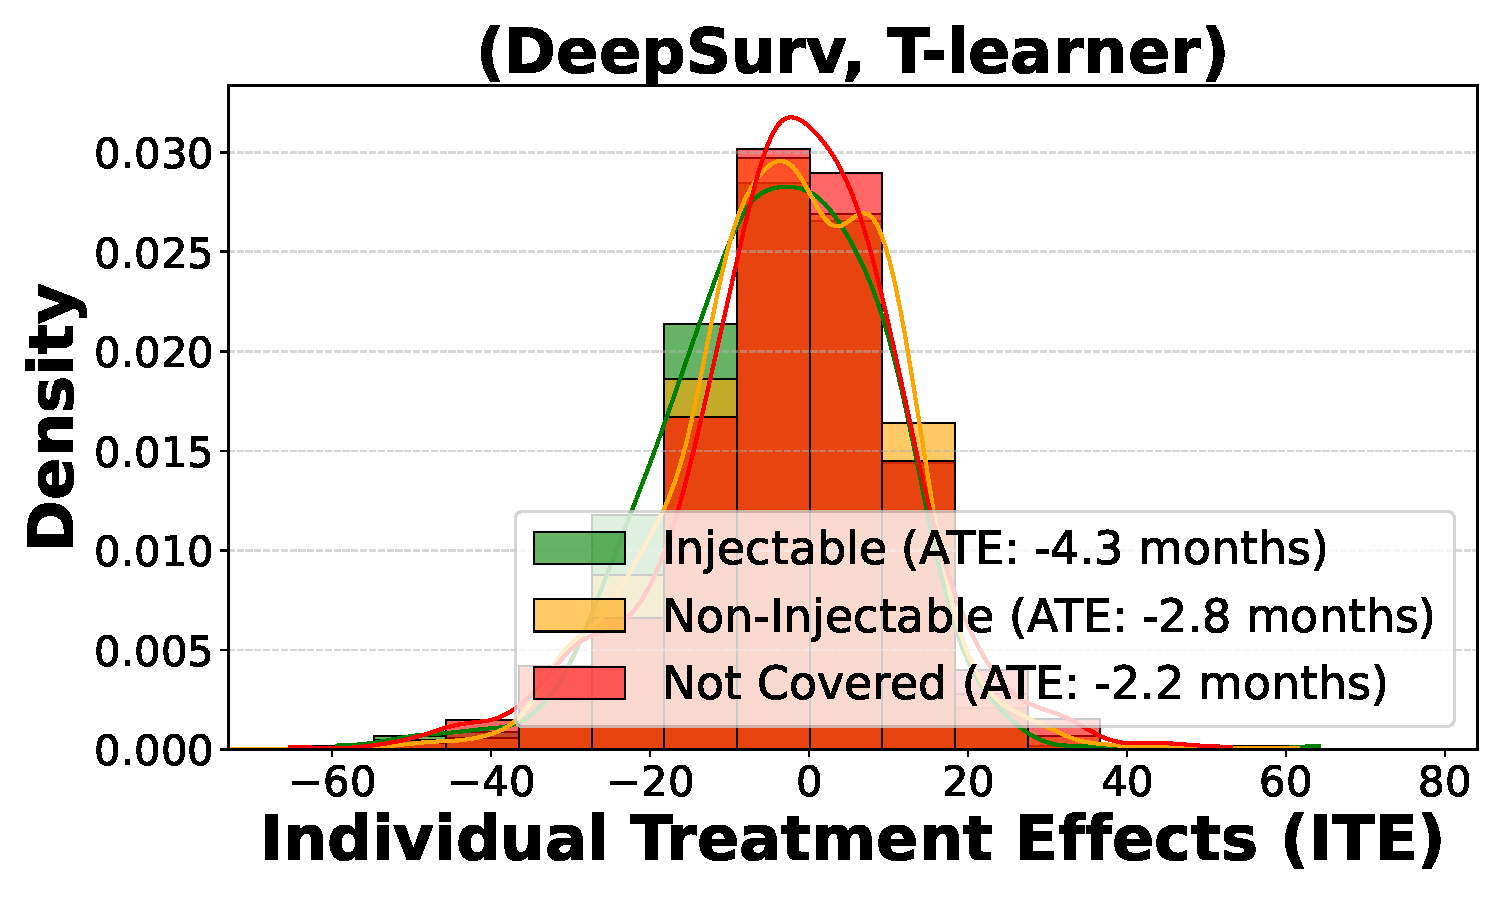
\includegraphics[width=.22\linewidth]{Chapters/chapter-03/images/ITE_injectable/ITE_DeepSurv_T-learner_injectable_type.pdf}}%
    \hfill
    \subfigure[\footnotesize (RandomSurvivalForest, T-Learner)]{\label{ch03:fig:ite_injectable_random_survival_forest}%
      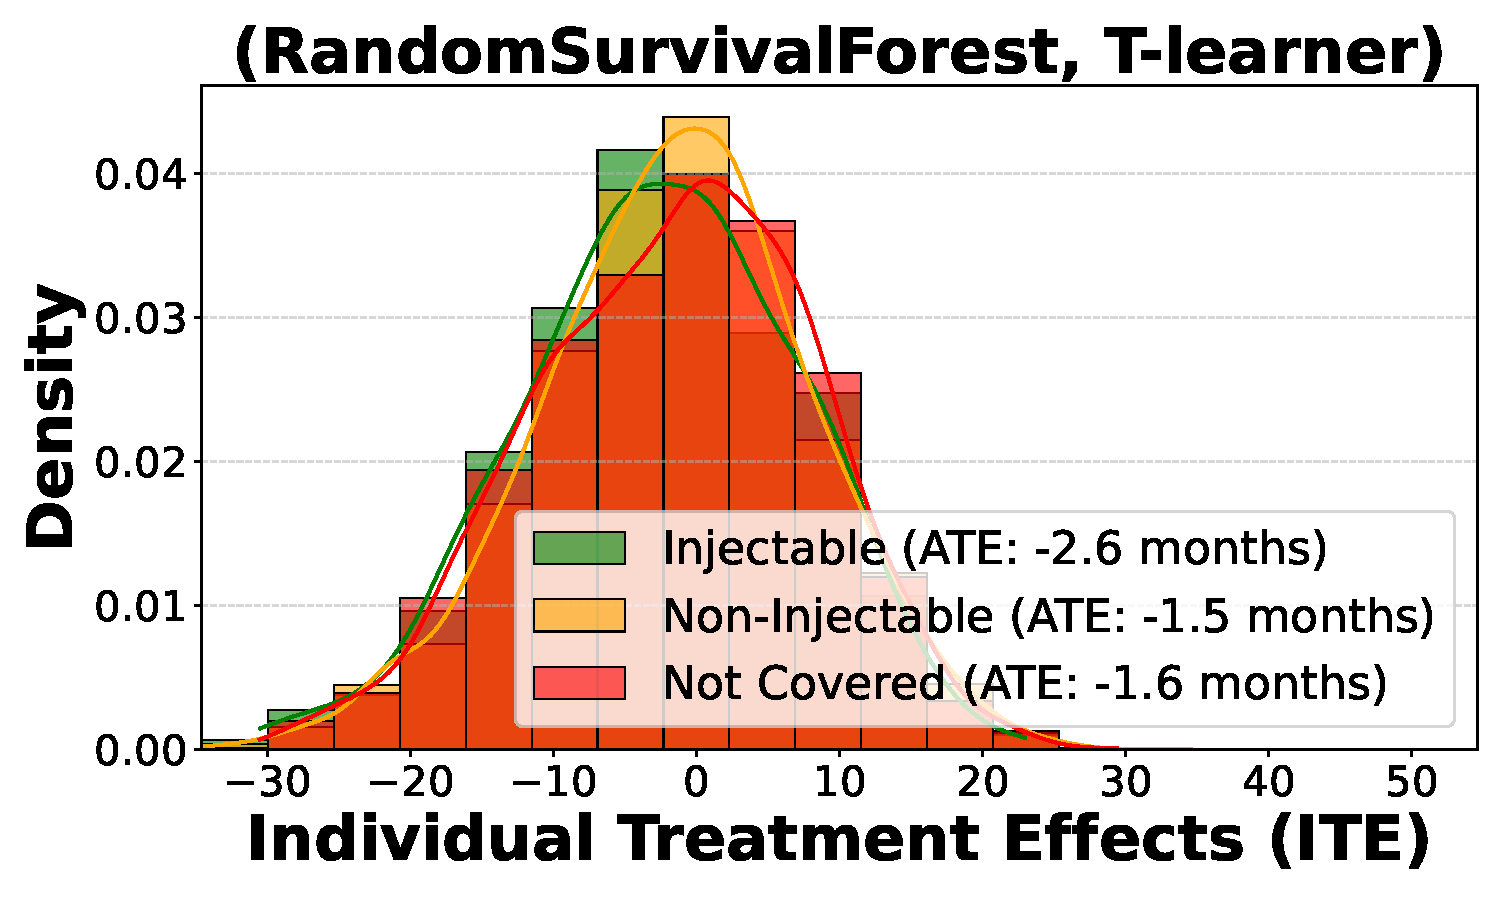
\includegraphics[width=.22\linewidth]{Chapters/chapter-03/images/ITE_injectable/ITE_RandomSurvivalForest_T-learner_injectable_type.pdf}}%
    \hfill
    \subfigure[\footnotesize CausalSurvivalForest]{\label{ch03:fig:ite_injectable_causal_survival_forest}%
      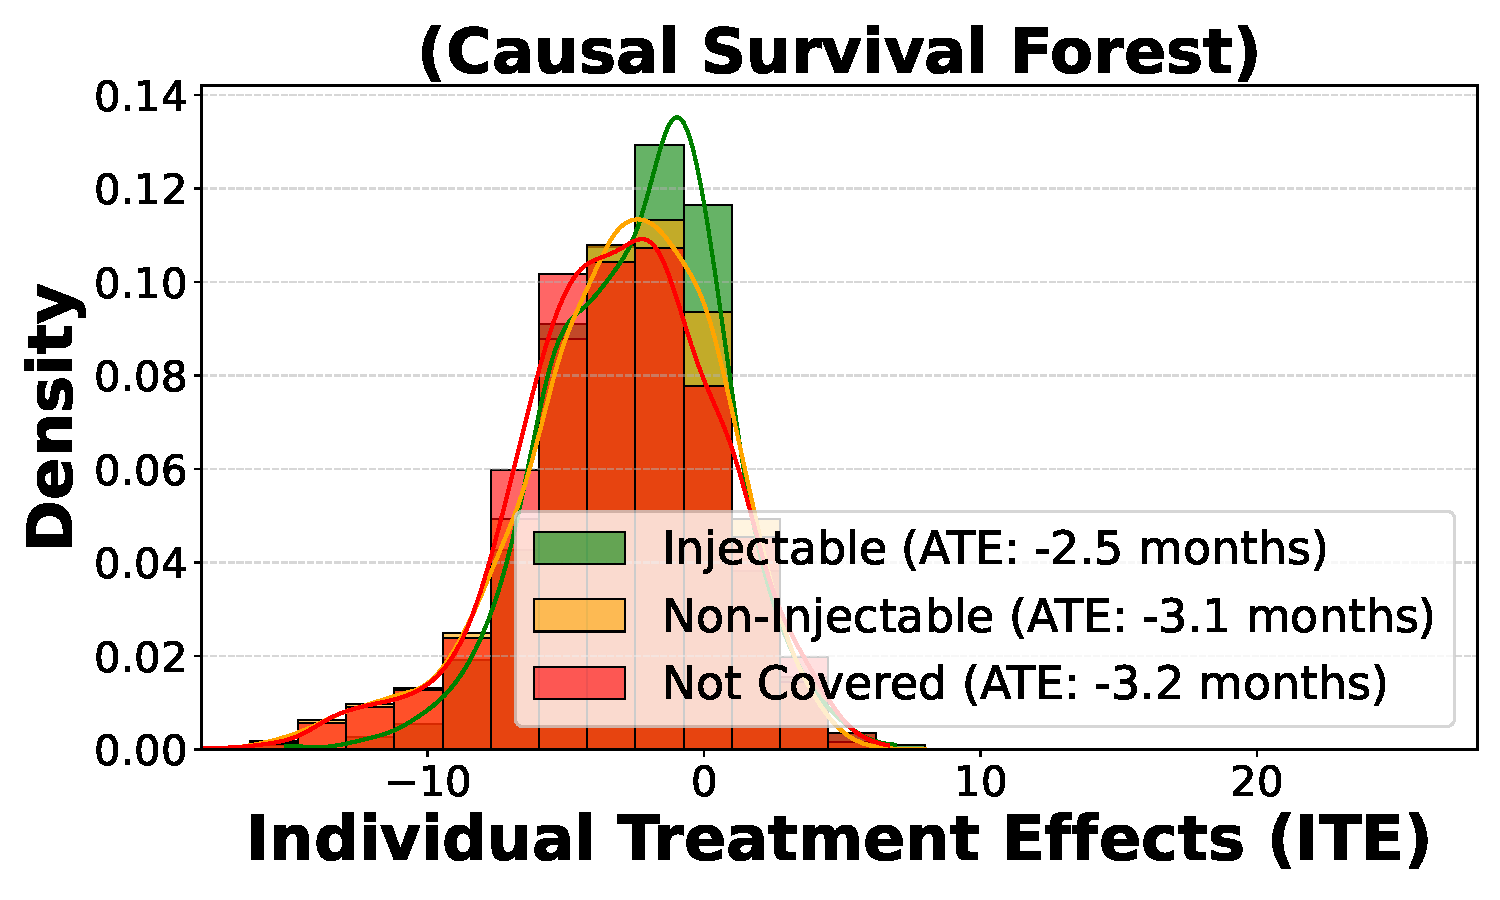
\includegraphics[width=.21\linewidth]{Chapters/chapter-03/images/ITE_injectable/ITE_CausalSurvivalForest_Causal_Survival_Forest_injectable_type.pdf}}%
  }
\end{figure}


By 12 months, some ATE estimates, including those from RSF and CSF, shift toward zero or even become positive. 
For instance, CSF reports an ATE of \(0.345 \pm 0.097\), suggesting that adverse event time differences between adherent and non-adherent groups diminish at later snapshots. 
Rather than reflecting a genuine weakening of the treatment effect, this trend likely arises from selection dynamics, as each snapshot only includes individuals who have not had an adverse event up to that point, potentially biasing the estimates toward a ``healthier'' subset. 
Additionally, residual time-varying confounding may contribute to this shift if certain survival-influencing factors are not fully accounted for in the estimators.

% \vspace{-1.5em}
